\documentclass{article}

\usepackage{graphicx}
\usepackage{tikz}
\usepackage{tikzsymbols}
\usetikzlibrary{calc,patterns,shapes.geometric}
\pagestyle{empty}
\usepackage[margin=0pt]{geometry}
\geometry{papersize={14in,12in}}

\def\centerarc[#1](#2)(#3:#4:#5){\draw[#1] ($(#2)+({#5*cos(#3)},{#5*sin(#3)})$) arc (#3:#4:#5);}

\begin{document}
	\begin{figure}
		\centering
		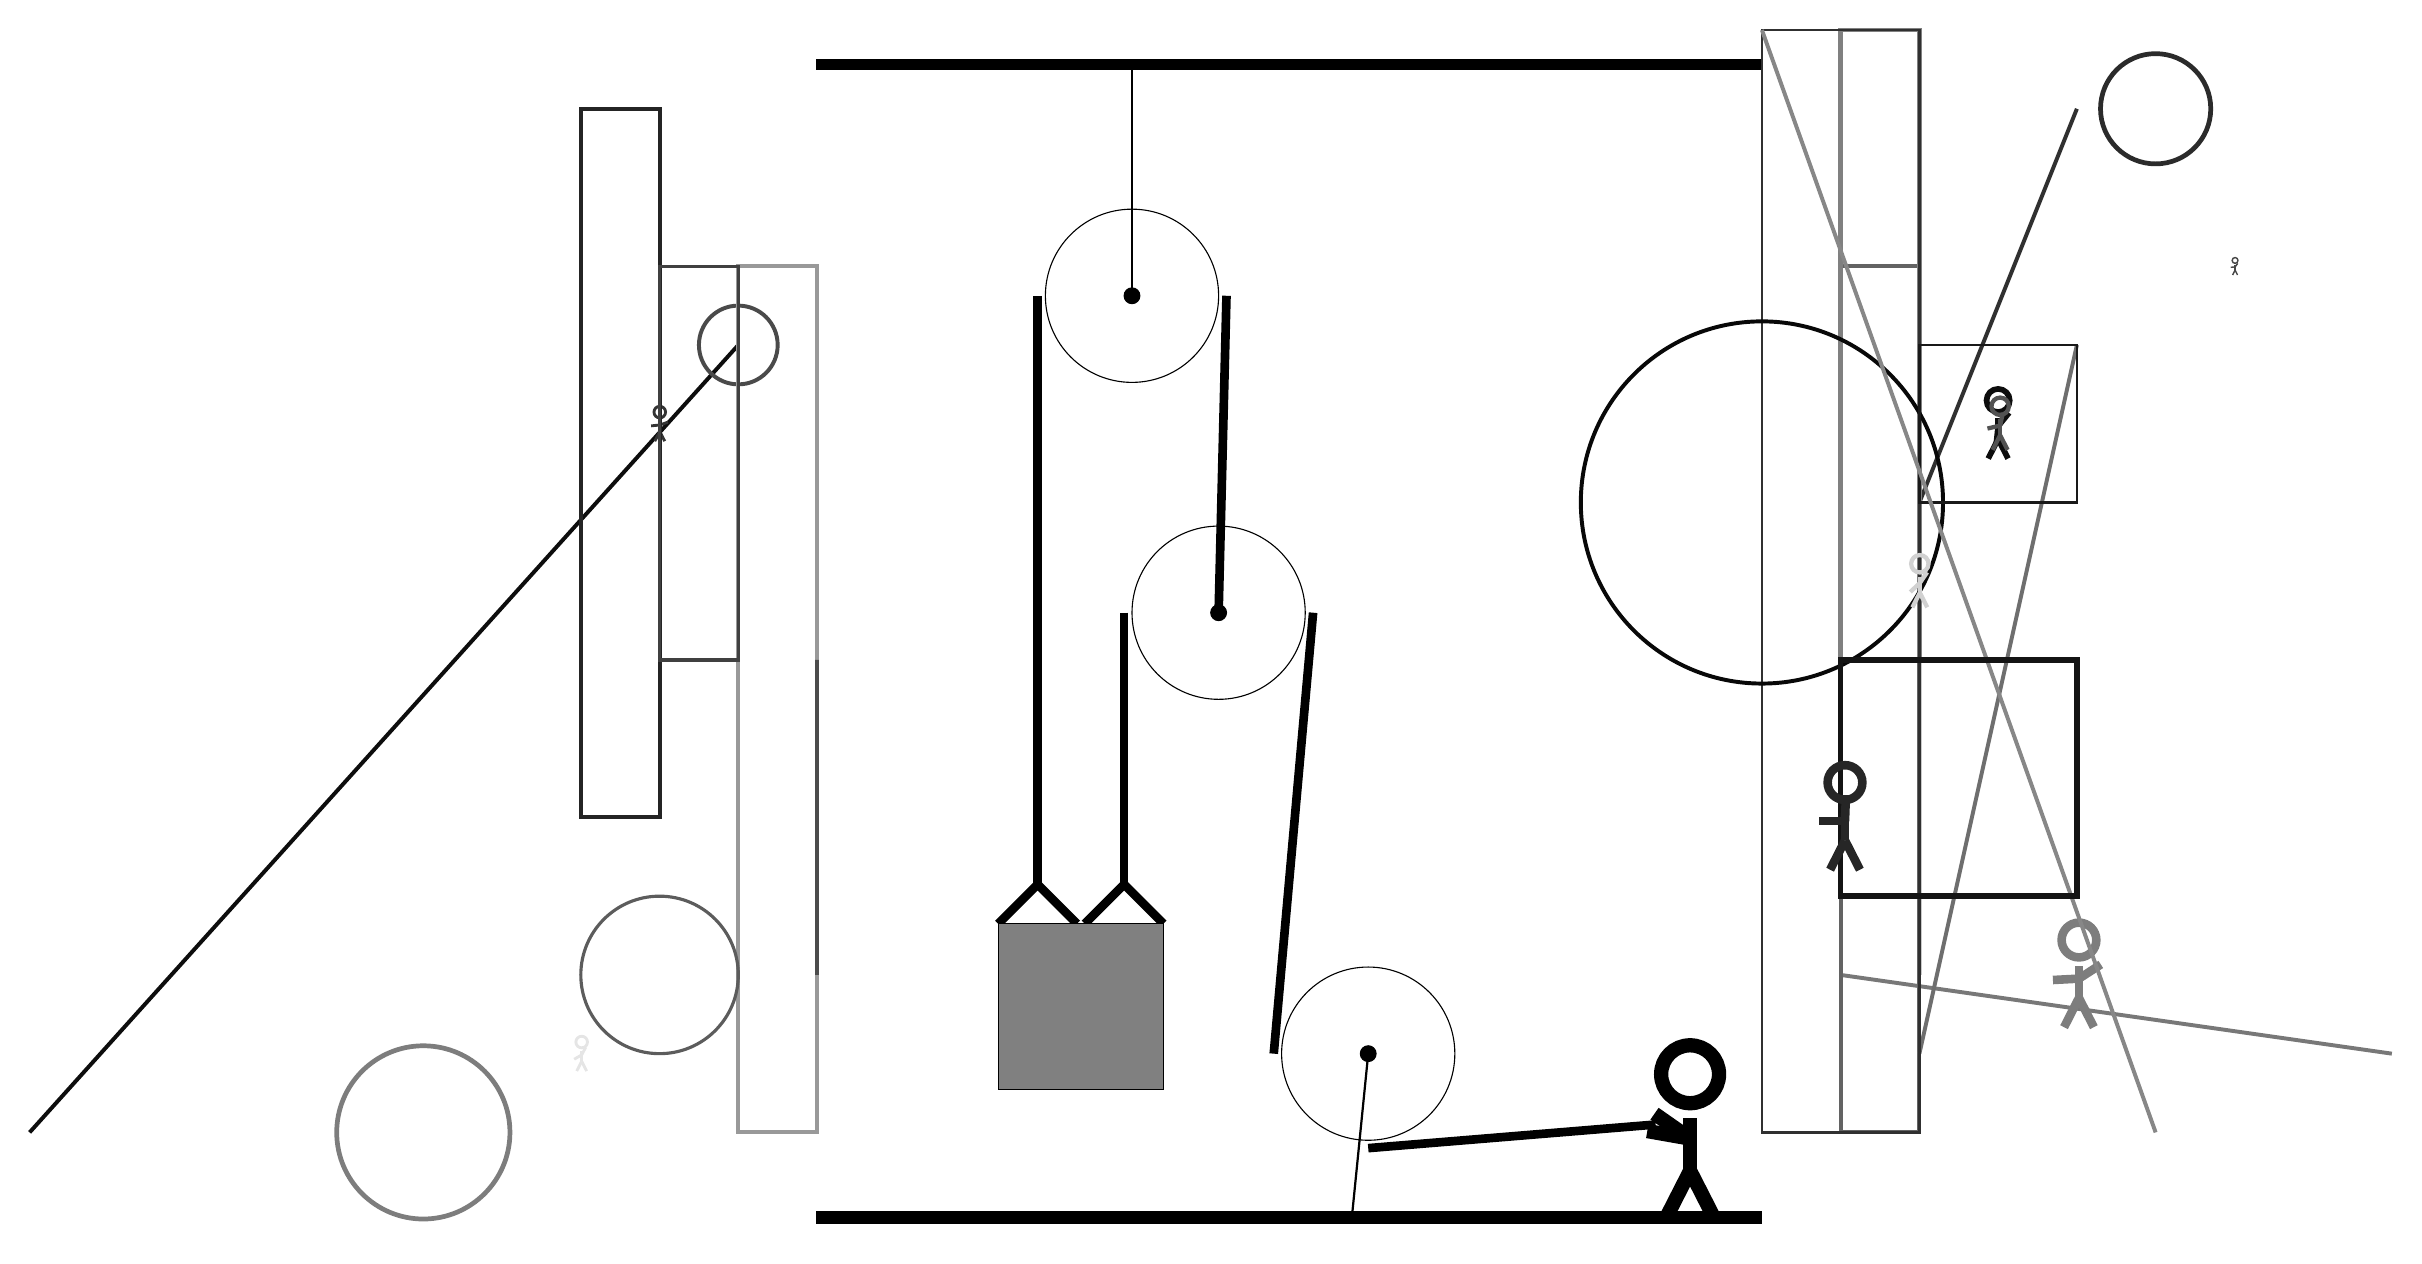
\begin{tikzpicture}
			%%%%% START %%%%%
			
			\draw[fill=black] (-2, 11.5) rectangle (10, 11.625);
			
			\draw (2, 8.625) circle (1.1);
			\draw[fill=black] (2, 8.625) circle (0.1);
			\draw[thick] (2, 8.625) -- (2, 11.5);
			
			\draw (3.1, 4.6) circle (1.1);
			\draw[fill=black] (3.1, 4.6) circle (0.1);
			
			\draw (5, -1) circle (1.1);
			\draw[fill=black] (5, -1) circle (0.1);
			\draw[thick] (5, -1) -- (4.8, -3);
			
			\draw[line width = 1.1mm]  (0.3, 0.65) -- (0.8, 1.15) -- (1.3, 0.65);
			\draw[line width = 1.1mm]  (1.4, 0.65) -- (1.9, 1.15) -- (2.4, 0.65);
			\draw[fill=black!50] (0.3, 0.65) rectangle (2.4, -1.45);
			
			\draw[line width = 1.1mm] (0.8, 8.625) -- (0.8, 1.15);
			\centerarc[line width = 1.1mm](2, 8.625)(0:180:1.2000000000000002);
			\draw[line width = 1.1mm] (3.2, 8.625) -- (3.1, 4.6);
			\draw[line width = 1.1mm] (1.9, 4.6) -- (1.9, 1.15);
			\centerarc[line width = 1.1mm](3.1, 4.6)(0:180:1.2000000000000002);
			\draw[line width = 1.1mm] (4.3, 4.6) -- (3.8, -1);
			\centerarc[line width = 1.1mm](5, -1)(180:270:1.2000000000000002);
			\draw[line width = 1.1mm] (5, -2.2) -- (8.65, -1.9);
			
			\draw[line width=0.5mm, color=black!53](11, 0) -- (18, -1);
			
			\draw [line width=0.6mm, color=black!83](15, 11) circle (0.7);
			\node[line width=0.5mm, color=black!51] at (14, 0) {\Strichmaxerl[6][3][33]};
			\node[line width=0.4mm, color=black!10] at (-5, -1) {\Strichmaxerl[2][30][62]};
			
			\draw[line width=0.5mm, color=black!81](12, 6) -- (14, 11);
			\draw[line width=0.7mm, color=black!21] (12, 0) rectangle (12, 11);
			
			\draw[line width=0.5mm, color=black!61] (11, 9) rectangle (12, -2);
			\draw[line width=0.5mm, color=black!57](14, 8) -- (12, -1);
			\draw[line width=0.5mm, color=black!95](-3, 8) -- (-12, -2);
			\node[line width=0.7mm, color=black!80] at (-4, 7) {\Strichmaxerl[2][6][19]};
			\draw[line width=0.6mm, color=black!50] (12, 4) rectangle (11, 12);
			\node[line width=0.2mm, color=black!95] at (13, 7) {\Strichmaxerl[4][84][51]};
			\draw[line width=0.5mm, color=black!86] (-4, 11) rectangle (-5, 2);
			
			\draw[line width=0.3mm, color=black!81] (10, 12) rectangle (12, -2);
			\draw [line width=0.5mm, color=black!97](10, 6) circle (2.3);
			\draw [line width=0.5mm, color=black!71](-3, 8) circle (0.5);
			
			\node[line width=0.7mm, color=black!18] at (12, 5) {\Strichmaxerl[3][43][56]};
			
			\draw[line width=0.5mm, color=black!40] (-2, 9) rectangle (-3, -2);
			\draw [line width=0.4mm, color=black!64](-4, 0) circle (1.0);
			
			\draw [line width=0.6mm, color=black!51](-7, -2) circle (1.1);
			\draw[line width=0.3mm, color=black!90] (12, 6) rectangle (14, 8);
			
			\node[line width=0.2mm, color=black!68] at (13, 7) {\Strichmaxerl[3][13][78]};
			\node[line width=0.4mm, color=black!72] at (16, 9) {\Strichmaxerl[1][6][53]};
			\draw[line width=0.5mm, color=black!47](10, 12) -- (15, -2);
			\draw[line width=0.4mm, color=black!75] (-4, 4) rectangle (-3, 9);
			
			\draw[line width=0.7mm, color=black!92] (11, 4) rectangle (14, 1);
			\draw[line width=0.6mm, color=black!70] (-2, 4) rectangle (-2, 0);
			\node[line width=0.5mm, color=black!85] at (11, 2) {\Strichmaxerl[6][0][88]};
			
			
			\node at (9, -2) {\Strichmaxerl[10][-35][170]};
			
			\draw[fill=black] (-2, -3) rectangle (10, -3.15);
			
			%%%%% END %%%%%
		\end{tikzpicture}
	\end{figure}	
\end{document}